\documentclass[]{book}
\usepackage{lmodern}
\usepackage{amssymb,amsmath}
\usepackage{ifxetex,ifluatex}
\usepackage{fixltx2e} % provides \textsubscript
\ifnum 0\ifxetex 1\fi\ifluatex 1\fi=0 % if pdftex
  \usepackage[T1]{fontenc}
  \usepackage[utf8]{inputenc}
\else % if luatex or xelatex
  \ifxetex
    \usepackage{mathspec}
  \else
    \usepackage{fontspec}
  \fi
  \defaultfontfeatures{Ligatures=TeX,Scale=MatchLowercase}
\fi
% use upquote if available, for straight quotes in verbatim environments
\IfFileExists{upquote.sty}{\usepackage{upquote}}{}
% use microtype if available
\IfFileExists{microtype.sty}{%
\usepackage{microtype}
\UseMicrotypeSet[protrusion]{basicmath} % disable protrusion for tt fonts
}{}
\usepackage[margin=1in]{geometry}
\usepackage{hyperref}
\hypersetup{unicode=true,
            pdftitle={htmlwidgets中文教程},
            pdfauthor={徐静 译},
            pdfborder={0 0 0},
            breaklinks=true}
\urlstyle{same}  % don't use monospace font for urls
\usepackage{natbib}
\bibliographystyle{apalike}
\usepackage{color}
\usepackage{fancyvrb}
\newcommand{\VerbBar}{|}
\newcommand{\VERB}{\Verb[commandchars=\\\{\}]}
\DefineVerbatimEnvironment{Highlighting}{Verbatim}{commandchars=\\\{\}}
% Add ',fontsize=\small' for more characters per line
\usepackage{framed}
\definecolor{shadecolor}{RGB}{248,248,248}
\newenvironment{Shaded}{\begin{snugshade}}{\end{snugshade}}
\newcommand{\KeywordTok}[1]{\textcolor[rgb]{0.13,0.29,0.53}{\textbf{#1}}}
\newcommand{\DataTypeTok}[1]{\textcolor[rgb]{0.13,0.29,0.53}{#1}}
\newcommand{\DecValTok}[1]{\textcolor[rgb]{0.00,0.00,0.81}{#1}}
\newcommand{\BaseNTok}[1]{\textcolor[rgb]{0.00,0.00,0.81}{#1}}
\newcommand{\FloatTok}[1]{\textcolor[rgb]{0.00,0.00,0.81}{#1}}
\newcommand{\ConstantTok}[1]{\textcolor[rgb]{0.00,0.00,0.00}{#1}}
\newcommand{\CharTok}[1]{\textcolor[rgb]{0.31,0.60,0.02}{#1}}
\newcommand{\SpecialCharTok}[1]{\textcolor[rgb]{0.00,0.00,0.00}{#1}}
\newcommand{\StringTok}[1]{\textcolor[rgb]{0.31,0.60,0.02}{#1}}
\newcommand{\VerbatimStringTok}[1]{\textcolor[rgb]{0.31,0.60,0.02}{#1}}
\newcommand{\SpecialStringTok}[1]{\textcolor[rgb]{0.31,0.60,0.02}{#1}}
\newcommand{\ImportTok}[1]{#1}
\newcommand{\CommentTok}[1]{\textcolor[rgb]{0.56,0.35,0.01}{\textit{#1}}}
\newcommand{\DocumentationTok}[1]{\textcolor[rgb]{0.56,0.35,0.01}{\textbf{\textit{#1}}}}
\newcommand{\AnnotationTok}[1]{\textcolor[rgb]{0.56,0.35,0.01}{\textbf{\textit{#1}}}}
\newcommand{\CommentVarTok}[1]{\textcolor[rgb]{0.56,0.35,0.01}{\textbf{\textit{#1}}}}
\newcommand{\OtherTok}[1]{\textcolor[rgb]{0.56,0.35,0.01}{#1}}
\newcommand{\FunctionTok}[1]{\textcolor[rgb]{0.00,0.00,0.00}{#1}}
\newcommand{\VariableTok}[1]{\textcolor[rgb]{0.00,0.00,0.00}{#1}}
\newcommand{\ControlFlowTok}[1]{\textcolor[rgb]{0.13,0.29,0.53}{\textbf{#1}}}
\newcommand{\OperatorTok}[1]{\textcolor[rgb]{0.81,0.36,0.00}{\textbf{#1}}}
\newcommand{\BuiltInTok}[1]{#1}
\newcommand{\ExtensionTok}[1]{#1}
\newcommand{\PreprocessorTok}[1]{\textcolor[rgb]{0.56,0.35,0.01}{\textit{#1}}}
\newcommand{\AttributeTok}[1]{\textcolor[rgb]{0.77,0.63,0.00}{#1}}
\newcommand{\RegionMarkerTok}[1]{#1}
\newcommand{\InformationTok}[1]{\textcolor[rgb]{0.56,0.35,0.01}{\textbf{\textit{#1}}}}
\newcommand{\WarningTok}[1]{\textcolor[rgb]{0.56,0.35,0.01}{\textbf{\textit{#1}}}}
\newcommand{\AlertTok}[1]{\textcolor[rgb]{0.94,0.16,0.16}{#1}}
\newcommand{\ErrorTok}[1]{\textcolor[rgb]{0.64,0.00,0.00}{\textbf{#1}}}
\newcommand{\NormalTok}[1]{#1}
\usepackage{longtable,booktabs}
\usepackage{graphicx,grffile}
\makeatletter
\def\maxwidth{\ifdim\Gin@nat@width>\linewidth\linewidth\else\Gin@nat@width\fi}
\def\maxheight{\ifdim\Gin@nat@height>\textheight\textheight\else\Gin@nat@height\fi}
\makeatother
% Scale images if necessary, so that they will not overflow the page
% margins by default, and it is still possible to overwrite the defaults
% using explicit options in \includegraphics[width, height, ...]{}
\setkeys{Gin}{width=\maxwidth,height=\maxheight,keepaspectratio}
\IfFileExists{parskip.sty}{%
\usepackage{parskip}
}{% else
\setlength{\parindent}{0pt}
\setlength{\parskip}{6pt plus 2pt minus 1pt}
}
\setlength{\emergencystretch}{3em}  % prevent overfull lines
\providecommand{\tightlist}{%
  \setlength{\itemsep}{0pt}\setlength{\parskip}{0pt}}
\setcounter{secnumdepth}{5}
% Redefines (sub)paragraphs to behave more like sections
\ifx\paragraph\undefined\else
\let\oldparagraph\paragraph
\renewcommand{\paragraph}[1]{\oldparagraph{#1}\mbox{}}
\fi
\ifx\subparagraph\undefined\else
\let\oldsubparagraph\subparagraph
\renewcommand{\subparagraph}[1]{\oldsubparagraph{#1}\mbox{}}
\fi

%%% Use protect on footnotes to avoid problems with footnotes in titles
\let\rmarkdownfootnote\footnote%
\def\footnote{\protect\rmarkdownfootnote}

%%% Change title format to be more compact
\usepackage{titling}

% Create subtitle command for use in maketitle
\newcommand{\subtitle}[1]{
  \posttitle{
    \begin{center}\large#1\end{center}
    }
}

\setlength{\droptitle}{-2em}
  \title{htmlwidgets中文教程}
  \pretitle{\vspace{\droptitle}\centering\huge}
  \posttitle{\par}
  \author{徐静 译}
  \preauthor{\centering\large\emph}
  \postauthor{\par}
  \predate{\centering\large\emph}
  \postdate{\par}
  \date{2018-07-04}

\usepackage{booktabs}
\usepackage{xeCJK}

\setCJKmainfont{宋体}

\setmainfont{Georgia}

\setromanfont{Georgia}

\setmonofont{Courier New}

\usepackage{amsthm}
\newtheorem{theorem}{Theorem}[chapter]
\newtheorem{lemma}{Lemma}[chapter]
\theoremstyle{definition}
\newtheorem{definition}{Definition}[chapter]
\newtheorem{corollary}{Corollary}[chapter]
\newtheorem{proposition}{Proposition}[chapter]
\theoremstyle{definition}
\newtheorem{example}{Example}[chapter]
\theoremstyle{definition}
\newtheorem{exercise}{Exercise}[chapter]
\theoremstyle{remark}
\newtheorem*{remark}{Remark}
\newtheorem*{solution}{Solution}
\begin{document}
\maketitle

{
\setcounter{tocdepth}{1}
\tableofcontents
}
\chapter*{声明}
\addcontentsline{toc}{chapter}{声明}

\href{https://CRAN.R-project.org/package=htmlwidgets}{htmlwidgets}是R语言中非常有划时代意义的包,因为有了htmlwidgets使得R语言在交互可视化和基于JavaScript的编程有了实质性的进步。htmlwidgets目前没有中文说明文档和教程,该文档是对官方文档的详细翻译,译者水平有限,读者可以在\url{https://github.com/DataXujing/htmlwidgets_CN/issues}中留言指正。

\begin{figure}
\centering
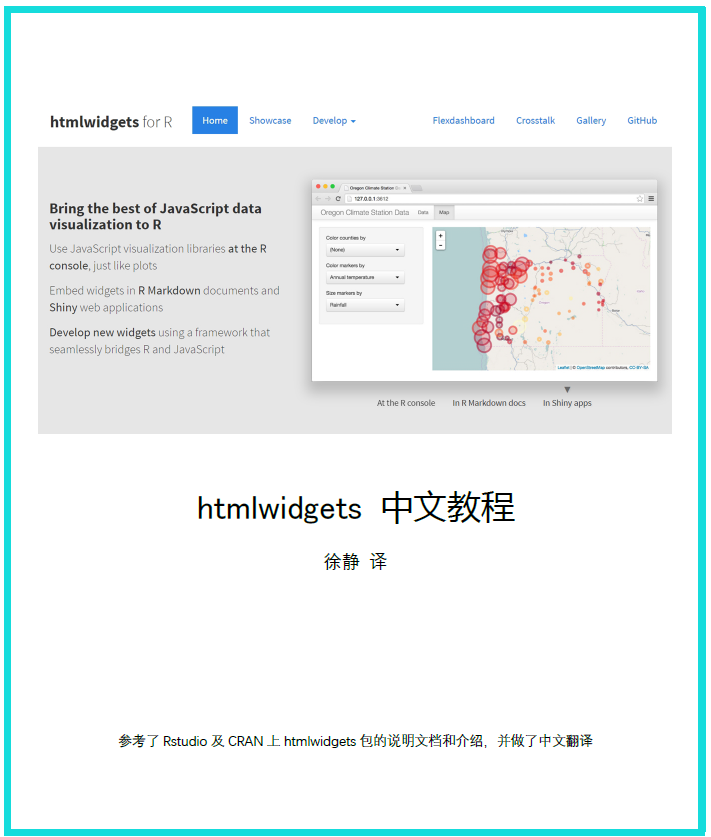
\includegraphics{pic/cover.png}
\caption{}
\end{figure}

\chapter*{序言}
\addcontentsline{toc}{chapter}{序言}

htmlwidgets,一个用来创建HTML控件的包,可以运行在R命令行, R Markdown,
Shiny。

\begin{verbatim}
Type Package
Title HTML Widgets for R
Version 1.2
Description A framework for creating HTML widgets that render in various
contexts including the R console, 'R Markdown' documents, and 'Shiny'
web applications.
License MIT + file LICENSE
VignetteBuilder knitr
Imports grDevices, htmltools (>= 0.3), jsonlite (>= 0.9.16), yaml
Suggests knitr (>= 1.8)
Enhances shiny (>= 1.0.5)
URL https://github.com/ramnathv/htmlwidgets
BugReports https://github.com/ramnathv/htmlwidgets/issues
RoxygenNote 6.0.1
NeedsCompilation no
Author Ramnath Vaidyanathan [aut, cph],Yihui Xie [aut],JJ Allaire [aut, cre],Joe Cheng [aut],
Kenton Russell [aut, cph],RStudio [cph]
Maintainer JJ Allaire <jj@rstudio.com>
Repository CRAN
Date/Publication 2018-04-19 12:43:03 UTC
\end{verbatim}

目前针对于htmlwidgets并没有详细的中文教程,译者会持续更新翻译htmlwidgets,并推出更多基于htmlwidgets的R包。

徐静

联信商务咨询有限公司

2018-07-02

\chapter*{关于译者}
\addcontentsline{toc}{chapter}{关于译者}

\textbf{徐静:}

硕士研究生,
目前的研究兴趣主要包括:数理统计,统计机器学习,深度学习,网络爬虫,前端可视化,R语言和Python语言的超级粉丝,多个R包和Python模块的作者,现在正逐步向Java迁移。

Graduate students,the current research interests include: mathematical
statistics, statistical machine learning, deep learning, web crawler,
front-end visualization. He is a super fan of R and Python, and the
author of several R packages and Python modules, and now gradually
migrating to Java.

\chapter{简介}\label{htmlwidgets-intro}

\section{概况}

\href{https://cran.r-project.org/web/packages/htmlwidgets/index.html}{htmlwidgets}包提供了一个R语言链接Javascript库的框架,HTML控件能够:

\begin{itemize}
\item
  在R命令中做分析比如方便的R作图
\item
  和R Markdown结合在一起
\item
  和shiny结合在一起
\item
  保存为独立的网页,通过电子邮件,Dropbox等ad-oc共享。
\end{itemize}

通过遵循一小部分易于遵循的约定,可以创建非常小的代码和HTML控件,所有控件包含如下部分:

\begin{enumerate}
\def\labelenumi{\arabic{enumi}.}
\item
  \emph{Dependencies}: 这些是控件用到的需要声明的Javascript和CSS
\item
  \emph{R binding}:
  这是终端用户将调用的功能,以向控件提供输入数据,并制定控件应该如何呈现各种选项,这包括在shiny应用程序中使用控件所需要的一些简短的样板功能。
\item
  \emph{javaScript binding}:
  这是JavaScript代码,把所有的东西粘在一起。将R绑定中收集的数据和选项传递给底层的JavaScript库
\end{enumerate}

已经有非常多的包基于htmlwidgets去完成,包括:

\begin{itemize}
\item
  leaflet -- 交互的地图绘制包
\item
  dygraphs -- 交互时间序列绘图包
\item
  networkD3 -- 基于D3.js的交互网络图可视化
\item
  sparkline -- 小型的内联图
\item
  DT -- 表格可视化
\item
  rthreejs -- 交互3D图
\end{itemize}

包的作者包括:Ramnath Vaidyanathan, Joe Cheng, JJ Allaire, Yihui Xie,
and Kenton Russell等。

HTML控件一般会寄存在一个R包中,并且应该包含他们的依赖关系的所有源代码,例如这里译者写的以个基于htmlwidgets的R包:\href{https://github.com/DataXujing/XuJIngd3plus}{XuJIngd3plus}。这是为了确保依赖的控件的完全可重复的(既不需要联网,也不需要运行服务器),说白了在你R包中,应该包含所有的源码包括你底层调用的JavaScript包或CSS。

\section{简单的开始}

如果你懂R语言和一点JavaScript,创建自己的小控件非常简单,最先要做的就是要安装htmlwidgets,在CRAN上:

\begin{Shaded}
\begin{Highlighting}[]
\KeywordTok{install.packages}\NormalTok{(}\StringTok{'htmlwidgets'}\NormalTok{)}
\end{Highlighting}
\end{Shaded}

你也可以在GitHub上安装开发版本:

\begin{Shaded}
\begin{Highlighting}[]
\NormalTok{devtools}\OperatorTok{::}\KeywordTok{install_github}\NormalTok{(}\StringTok{'ramnathv/htmlwidgets'}\NormalTok{)}
\end{Highlighting}
\end{Shaded}

通过包中自带的说明文档,让你快速的熟悉htmlwidgets并进入开发者状态,包括:

\begin{itemize}
\item
  Introduction to HTML Widgets
\item
  HTML Widget Sizing
\item
  HTML Widgets: Advanced Topics
\end{itemize}

我们会持续把他们翻译成中文,让中国人看起来更爽。

\section{例子(sigma.js)}\label{sigma.js}

首先,我们将通过创建一个控件来封装\href{http://sigmajs.org/}{sigma.js}图形可视化库。当我们完成后,我们可以用来显示\href{https://gephi.org/gexf/format/}{GEXF}(Graph
Exchange XML Format)数据文件的交互可视化,例如:

\begin{Shaded}
\begin{Highlighting}[]
\KeywordTok{library}\NormalTok{(sigma)}
\NormalTok{data <-}\StringTok{ }\KeywordTok{system.file}\NormalTok{(}\StringTok{"examples/ediaspora.gexf.xml"}\NormalTok{, }\DataTypeTok{package =} \StringTok{"sigma"}\NormalTok{)}
\KeywordTok{sigma}\NormalTok{(data)}
\end{Highlighting}
\end{Shaded}

\begin{figure}
\centering
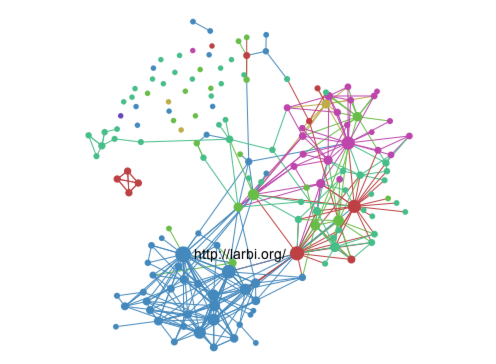
\includegraphics{pic/ch1_1.png}
\caption{}
\end{figure}

注意上面的输出仅仅是一个静态图像,你可以按照下文的Demo做一个交互的版本。

创建这种绑定所需的代码非常少。下面我们将一步一步地介绍所有的控件。然后,我们将描述如何创建自己的控件(包括为所有核心组件自动生成基本的脚手架)。

\subsection{文件布局}

假设我们的控件被命名为\textbf{sigma},并且位于同名的R包中。我们的JavaScript绑定源代码文件名为sigma.js。由于我们的控件将读取GEXF数据文件,我们还需要包括基础sigma.min.js库以及GEXF插件,下面是我们将添加到包中的文件:

\begin{verbatim}
R/
| sigma.R

inst/
|-- htmlwidgets/
|   |-- sigma.js
|   |-- sigma.yaml
|   |-- lib/
|   |   |-- sigma-1.0.3/
|   |   |   |-- sigma.min.js
|   |   |   |-- plugins/
|   |   |   |   |-- sigma.parsers.gexf.min.js
\end{verbatim}

请注意,JavaScript,YAML和其他依赖项都包含在inst/htmlwidgets目录中(随后将被安装到一个名为htmlwidgets的包的子目录中)。

\subsection{依赖关系}

依赖项是控件使用的JavaScript和CSS资源。依赖项包含在inst/htmlwidgets/lib目录中。依赖关系是使用YAML配置文件指定的,该文件使用控件的名称作为其基本文件名。以下是我们的sigma.yaml文件的样子

\begin{verbatim}
dependencies:
  - name: sigma
    version: 1.0.3
    src: htmlwidgets/lib/sigma-1.0.3
    script: 
      - sigma.min.js
      - plugins/sigma.parsers.gexf.min.js
\end{verbatim}

依赖关系src详述了引用目录,包含库和指定的JavaScript代码文件。如果包含多个JS脚本,每一个占每一行,并且以`-开头。同时你可以天剑stylesheet条目,还有元条目或头条目,多依赖关系可以在一个YAML文件中声明,更多的请参考htmlDependency函数,该函数在\href{https://cran.r-project.org/web/packages/htmltools/index.html}{htmltools}包中

\subsection{R绑定(R binding)}\label{rr-binding}

我们需要为用户提供一个调用我们的控件的R函数。通常,该函数将接受输入数据以及控制控件的显示的各种选项。下面是sigma的R函数:

\begin{Shaded}
\begin{Highlighting}[]
\CommentTok{#' @import htmlwidgets}
\CommentTok{#' @export}
\NormalTok{sigma <-}\StringTok{ }\ControlFlowTok{function}\NormalTok{(gexf, }\DataTypeTok{drawEdges =} \OtherTok{TRUE}\NormalTok{, }\DataTypeTok{drawNodes =} \OtherTok{TRUE}\NormalTok{,}
                  \DataTypeTok{width =} \OtherTok{NULL}\NormalTok{, }\DataTypeTok{height =} \OtherTok{NULL}\NormalTok{) \{}
  
  \CommentTok{# read the gexf file}
\NormalTok{  data <-}\StringTok{ }\KeywordTok{paste}\NormalTok{(}\KeywordTok{readLines}\NormalTok{(gexf), }\DataTypeTok{collapse=}\StringTok{"}\CharTok{\textbackslash{}n}\StringTok{"}\NormalTok{)}
  
  \CommentTok{# create a list that contains the settings}
\NormalTok{  settings <-}\StringTok{ }\KeywordTok{list}\NormalTok{(}
    \DataTypeTok{drawEdges =}\NormalTok{ drawEdges,}
    \DataTypeTok{drawNodes =}\NormalTok{ drawNodes}
\NormalTok{  )}
  
  \CommentTok{# pass the data and settings using 'x'}
\NormalTok{  x <-}\StringTok{ }\KeywordTok{list}\NormalTok{(}
    \DataTypeTok{data =}\NormalTok{ data,}
    \DataTypeTok{settings =}\NormalTok{ settings}
\NormalTok{  )}
  
  \CommentTok{# create the widget}
\NormalTok{  htmlwidgets}\OperatorTok{::}\KeywordTok{createWidget}\NormalTok{(}\StringTok{"sigma"}\NormalTok{, x, }\DataTypeTok{width =}\NormalTok{ width, }\DataTypeTok{height =}\NormalTok{ height)}
\NormalTok{\}}
\end{Highlighting}
\end{Shaded}

函数包含两类输入:GEXF数据文件和一些附加的设置参数用来控制如何显示图片。这些输入都集中在一个叫做x的列表中,然后灌入到htmlwidgets::createWidget函数。这个x变量随后将被用于sigma的JavaScript绑定(下面将对此进行描述),指定的任何宽度或高度参数也会被转发到widget(默认情况下,控件自动调整大小,因此通常不需要显式的宽度或高度)。

我们也希望sigma控件能够在shiny应用中使用,因此我们添加了下面的公式化的shiny
output和render函数(对于所有的控件来说,它总是相同的)

\begin{Shaded}
\begin{Highlighting}[]
\CommentTok{#' @export}
\NormalTok{sigmaOutput <-}\StringTok{ }\ControlFlowTok{function}\NormalTok{(outputId, }\DataTypeTok{width =} \StringTok{"100%"}\NormalTok{, }\DataTypeTok{height =} \StringTok{"400px"}\NormalTok{) \{}
\NormalTok{  htmlwidgets}\OperatorTok{::}\KeywordTok{shinyWidgetOutput}\NormalTok{(outputId, }\StringTok{"sigma"}\NormalTok{, width, height, }\DataTypeTok{package =} \StringTok{"sigma"}\NormalTok{)}
\NormalTok{\}}
\CommentTok{#' @export}
\CommentTok{#https://blog.csdn.net/songzhilian22/article/details/49487467}
\NormalTok{renderSigma <-}\StringTok{ }\ControlFlowTok{function}\NormalTok{(expr, }\DataTypeTok{env =} \KeywordTok{parent.frame}\NormalTok{(), }\DataTypeTok{quoted =} \OtherTok{FALSE}\NormalTok{) \{}
  \ControlFlowTok{if}\NormalTok{ (}\OperatorTok{!}\NormalTok{quoted) \{ expr <-}\StringTok{ }\KeywordTok{substitute}\NormalTok{(expr) \} }\CommentTok{# force quoted}
\NormalTok{  htmlwidgets}\OperatorTok{::}\KeywordTok{shinyRenderWidget}\NormalTok{(expr, sigmaOutput, env, }\DataTypeTok{quoted =} \OtherTok{TRUE}\NormalTok{)}
\NormalTok{\}}
\end{Highlighting}
\end{Shaded}

\subsection{JavaScript绑定(JavaScript
binding)}\label{javascriptjavascript-binding}

注意:在htmlwidgets0.5.2和更早的版本中使用了一个更老、更不直观的JavaScript绑定API,并在htmlwidgets的更新版本中继续支持。有关遗留绑定API的详细信息,请参见此归档版本。新的控件件被鼓励使用下面描述的更新的API。谜题中的第三个部分是激活控件所需的JavaScript。按照惯例,我们将在文件inst/htmlwidgets/sigma.js中定义JavaScript绑定。下面是绑定的完整源代码:

\begin{verbatim}
HTMLWidgets.widget({

  name: "sigma",
  
  type: "output",
  
  factory: function(el, width, height) {
  
    // create our sigma object and bind it to the element
    var sig = new sigma(el.id);
    
    return {
      renderValue: function(x) {
          
        // parse gexf data
        var parser = new DOMParser();
        var data = parser.parseFromString(x.data, "application/xml");
        
        // apply settings
        for (var name in x.settings)
          sig.settings(name, x.settings[name]);
        
        // update the sigma object
        sigma.parsers.gexf(
          data,          // parsed gexf data
          sig,           // sigma object
          function() {
            // need to call refresh to reflect new settings and data
            sig.refresh();
          }
        );
      },
      
      resize: function(width, height) {
        
        // forward resize on to sigma renderers
        for (var name in sig.renderers)
          sig.renderers[name].resize(width, height);  
      },
      
      // Make the sigma object available as a property on the widget
      // instance we're returning from factory(). This is generally a
      // good idea for extensibility--it helps users of this widget
      // interact directly with sigma, if needed.
      s: sig
    };
  }
});
\end{verbatim}

我们为控件提供了名称和类型,再加上一个工厂函数,它采用el(将承载这控件的HTML元素)、宽度和高度(HTML元素的宽度和高度,以像素为单位),您总是可以使用OffStStand宽度和OffSETHEE来实现这一点。

工厂函数要准备启动接收HTML元素的值。在这个案例,我们创建一个新的sigma元素和把它的DOM元素的ID,承载页面的控件。

我们稍后需要访问sigma对象(以更新它的数据和设置),因此我们将其保存为变量sig。请注意,直接在工厂函数内部声明的变量与特定的控件实例/el绑定。

工厂函数的返回值被称为控件实例对象。它是htmlwidgets运行时和正在包装的JavaScript可视化之间的桥梁。顾名思义,每个控件实例对象负责管理页面上的单个控件实例。

您创建的控件实例对象必须有一个所需的方法,并且可以有一个可选的方法:

\begin{enumerate}
\def\labelenumi{\arabic{enumi}.}
\item
  所需的renderValue方法实际上将动态数据和设置填充到WEB的DOM元素中。x包含控件数据和设置。我们解析和更新GEXF数据,将设置应用到我们先前创建的sig
  Sigma对象,最后调用刷新以反映屏幕上的新值。这种方法可以重复调用不同的数据(例如:在shiny中),所以一定要考虑到这种可能性。如果它对你的控件有意义,
  考虑使您的可视化转换顺利地从x的一个值开始到另一个。
\item
  每当包含控件的元素被调整大小时,就会调用可选的大小调整方法。不执行此方法的唯一原因是如果您的控件自然缩放(当它的元素大小改变时不需要附加的JavaScript代码)。在sigma
  .js的情况下,我们将大小调整信息转发给每个底层sigma渲染器。
\end{enumerate}

所有JavaScript库都处理初始化、绑定到DOM元素、动态更新数据和稍微不同地调整大小。创建控件的JavaScript方面的大部分工作是将这三个函数工厂、渲染值和大小正确地映射到底层库的行为。sigma.js示例使用一个简单的对象文字来创建它的控件实例对象,但是您也可以使用基于类的对象或任何其他样式的对象,只要obj.renderValue(x)和obj.resize(width,
height)(宽度,高度)可以调用它。

可以在控件实例对象上添加其他方法和属性。虽然它们不会被htmlwidgets本身调用,但它们可能对知道一些JavaScript的控件的用户有用,并希望通过添加自定义JS代码(例如使用htmlwidgets::onRender
R函数)来进一步定制您的控件。在这种情况下,我们添加一个s属性,使sigma对象本身可用。

\subsection{演示}

我们的控件现在完成了!如果您想在不重放所有代码的情况下测试它,您可以从GitHub安装它如下:

\begin{Shaded}
\begin{Highlighting}[]
\NormalTok{devtools}\OperatorTok{::}\KeywordTok{install_github}\NormalTok{(}\StringTok{'jjallaire/sigma'}\NormalTok{)}
\end{Highlighting}
\end{Shaded}

下面是代码的示例,其中包含了包中包含的一些示例数据:

\begin{Shaded}
\begin{Highlighting}[]
\KeywordTok{library}\NormalTok{(sigma)}
\KeywordTok{sigma}\NormalTok{(}\KeywordTok{system.file}\NormalTok{(}\StringTok{"examples/ediaspora.gexf.xml"}\NormalTok{, }\DataTypeTok{package =} \StringTok{"sigma"}\NormalTok{))}
\end{Highlighting}
\end{Shaded}

如果在R控制台中执行此代码,您将看到在RStudio
Viewer中显示的控件(或者如果不运行RStudio,则在外部浏览器中)。如果将其包含在R
Markdown文档中,则窗口控件将嵌入到文档中。

我们还可以在shiny应用程序中使用控件:

\begin{Shaded}
\begin{Highlighting}[]
\KeywordTok{library}\NormalTok{(shiny)}
\KeywordTok{library}\NormalTok{(sigma)}

\NormalTok{gexf <-}\StringTok{ }\KeywordTok{system.file}\NormalTok{(}\StringTok{"examples/ediaspora.gexf.xml"}\NormalTok{, }\DataTypeTok{package =} \StringTok{"sigma"}\NormalTok{)}

\NormalTok{ui =}\StringTok{ }\KeywordTok{shinyUI}\NormalTok{(}\KeywordTok{fluidPage}\NormalTok{(}
  \KeywordTok{checkboxInput}\NormalTok{(}\StringTok{"drawEdges"}\NormalTok{, }\StringTok{"Draw Edges"}\NormalTok{, }\DataTypeTok{value =} \OtherTok{TRUE}\NormalTok{),}
  \KeywordTok{checkboxInput}\NormalTok{(}\StringTok{"drawNodes"}\NormalTok{, }\StringTok{"Draw Nodes"}\NormalTok{, }\DataTypeTok{value =} \OtherTok{TRUE}\NormalTok{),}
  \KeywordTok{sigmaOutput}\NormalTok{(}\StringTok{'sigma'}\NormalTok{)}
\NormalTok{))}

\NormalTok{server =}\StringTok{ }\ControlFlowTok{function}\NormalTok{(input, output) \{}
\NormalTok{  output}\OperatorTok{$}\NormalTok{sigma <-}\StringTok{ }\KeywordTok{renderSigma}\NormalTok{(}
    \KeywordTok{sigma}\NormalTok{(gexf, }
          \DataTypeTok{drawEdges =}\NormalTok{ input}\OperatorTok{$}\NormalTok{drawEdges, }
          \DataTypeTok{drawNodes =}\NormalTok{ input}\OperatorTok{$}\NormalTok{drawNodes)}
\NormalTok{  )}
\NormalTok{\}}

\KeywordTok{shinyApp}\NormalTok{(}\DataTypeTok{ui =}\NormalTok{ ui, }\DataTypeTok{server =}\NormalTok{ server)}
\end{Highlighting}
\end{Shaded}

\section{创建你自己的widgets}\label{widgets}

\subsection{需求(Requirements)}\label{requirements}

要实现一个控件,您需要创建一个新的R包,而这又取决于htmlwidgets包。可以在CRAN中安装:

\begin{Shaded}
\begin{Highlighting}[]
\KeywordTok{install.packages}\NormalTok{(}\StringTok{"htmlwidgets"}\NormalTok{)}
\end{Highlighting}
\end{Shaded}

\subsection{脚手架(Scaffolding)}\label{scaffolding}

要创建一个新的控件,可以调用\textbf{scaffoldWidget}函数来生成控件的基本结构。函数将:

\begin{itemize}
\item
  创建.R,.js,.yaml等控件需要的文件
\item
  如果提供,取一个\href{https://bower.io/}{Bower}包名称并自动下载JavaScript库(及其依赖项),并将所需的条目添加到.yaml文件中。
\end{itemize}

这个方法是非常推荐的,因为它确保你开始使用正确的文件结构。
下面是一个示例,假设您希望在一个新的同名包中创建名为``mywidget''的小部件:

\begin{Shaded}
\begin{Highlighting}[]
\NormalTok{devtools}\OperatorTok{::}\KeywordTok{create}\NormalTok{(}\StringTok{"mywidget"}\NormalTok{)               }\CommentTok{# create package using devtools}
\KeywordTok{setwd}\NormalTok{(}\StringTok{"mywidget"}\NormalTok{)                          }\CommentTok{# navigate to package dir}
\NormalTok{htmlwidgets}\OperatorTok{::}\KeywordTok{scaffoldWidget}\NormalTok{(}\StringTok{"mywidget"}\NormalTok{)    }\CommentTok{# create widget scaffolding}
\NormalTok{devtools}\OperatorTok{::}\KeywordTok{install}\NormalTok{()  }
\end{Highlighting}
\end{Shaded}

这将创建一个简单的控件,它使用单个文本参数,并在控件HTML元素中显示该文本。你可以这样试试:

\begin{Shaded}
\begin{Highlighting}[]
\KeywordTok{library}\NormalTok{(mywidget)}
\KeywordTok{mywidget}\NormalTok{(}\StringTok{"hello, world"}\NormalTok{)}
\end{Highlighting}
\end{Shaded}

这是最可能的控件,并且还没有包含一个JavaScript库来连接(注意,scaffoldWidget可以可选地包含通过JavaScript库依赖关系的bowerPkg参数)这是最可能的小部件,并且还没有包含一个JavaScript库来连接(注意,scaffoldWidget可以可选地包含通过JavaScript库依赖关系的bowerPkg参数)。
在开始开发之前,您应该查看上面的介绍性示例,以确保您理解各个组件,并在下一节中查看与文章相关联的附加文章和示例。

\subsection{更多}

\subsubsection{其他}

还有更多的文章覆盖更高级的领域:

\begin{itemize}
\item
  HTML Widget
  Sizing:解释自定义大小调整策略以及何时可能需要使用它们,并描述在JavaScript绑定中实现调整大小的方法。
\item
  HTML Widgets: Advanced
  Topics:描述支持每个控件实例数据、数据转换(例如,将数据帧转换为D3数据集)以及提供live
  JavaScript对象(例如函数定义)的控件选项的框架特征。
\end{itemize}

当大多数JavaScript库需要一些额外的交互以保持它们的大小与它们的包含元素同步时,HTML
Widget Sizing就显得尤为重要。

\subsubsection{例子}

学习其他包的代码是了解更多关于创建小部件的一个好方法:

\begin{itemize}
\item
  \href{https://CRAN.R-project.org/package=networkD3}{networkD3}
\item
  \href{https://CRAN.R-project.org/package=dygraphs}{dygraphs}
\item
  \href{https://github.com/htmlwidgets/sparkline}{sparkline}
\end{itemize}

\subsubsection{问题}

如果您对开发控件或开发过程中遇到的问题有疑问,请毫不犹豫地在项目的GitHub存储库上发布一个问题。

\chapter{HTML空间尺寸调整}\label{htmlwidgets-Sizing}

\section{概述}

在HTML控件的工作中,就像R中的绘图(plot),HTML控件智能的将他们自己的大小放在容器中,无论是在Rstudio
Viewer中,knitr中的图还是在Shiny
UI中的面板。\textbf{htmlwidgets}框架提供了一种丰富的机制来指定控件的大小调整行为。

这种大小调整机制是为了解决影响控件的自然尺寸的以下约束:

\begin{itemize}
\item
  \textbf{The kind of widget it
  is}.有些控件可能仅仅需要设计成小的,固定尺寸(例如\href{https://github.com/htmlwidgets/sparkline}{sparkline}),而有些控件可能需要基于像素点做不断地调整(例如\href{http://christophergandrud.github.io/networkD3/}{network
  graphs})
\item
  \textbf{The context into which the widget is rendered.}有些控件在R
  Markdown中看起来是以
  \(980px \times 480px\),相同的控件在Rstudio的Viewer中看起来要小的多。
\end{itemize}

分两步处理控件的大小:

\begin{enumerate}
\def\labelenumi{\arabic{enumi}.}
\item
  首先为控件指定大小调整策略,这是通过createWidget函数中的sizingPolicy参数实现的。大多数控件可以接受默认的大小调整策略((或者只覆盖其中的一个或两个方面)并获得满意的大小调整行为(详见下文)。)
\item
  框架使用大小调整策略来计算给定的窗口中所呈现的窗口的正确宽度和高度。然后将其大小信息传递给控件JavaScript绑定的初始化和调整大小方法。控件将大小的信息传递给底层的JS库。
\end{enumerate}

\section{指定大小调整策略}

\chapter{HTML控件:高级主题}\label{htmlwidgets-advanced}

正在翻译中\ldots{}

\chapter{htmlwidgets包中函数的总结}\label{htmlwidgets-pkgintro}

正在翻译中\ldots{}

\chapter{总结}\label{summary}

总结

\chapter{参考文献}\label{reference}

{[}1{]}.
\href{https://github.com/ramnathv/htmlwidgets}{GitHub上htmlwidgets的地址}

{[}2{]}.
\href{https://CRAN.R-project.org/package=htmlwidgets}{CRAN上htmlwidgets的地址}

{[}3{]}. \href{https://www.htmlwidgets.org/}{Rstudio官网上的地址}

\bibliography{book.bib,packages.bib}


\end{document}
